\section{Optimierung der Parameter des Neuronalen Netzes}
Als (künstliches) Neuronales Netz wird im Allgemeinen jede Annsammlung von verbundenen Neuronen bezeichnet, die ein individuelles Ansprechverhalten zu einem gegebenen Input Signal aufweisen. Das Neuronale Netz besteht meist aus mehreren Schichten (HiddenLayers), wobei die erste Schicht Input Neuronen und die letzte die Output Neuronen darstellen. In unserem Fall besteht das Output-layer aus lediglich einem Neuron, da nur zwischen Signal und Background unterschieden werden muss.\\ \\
Um die Zeit zu verringern, die das NN benötigt um die Daten zu trainieren, wurde teilweise mit der Option Sampling=0.X gearbeitet, welche nur den X-ten Anteil der Trainings- und Testdatensätze verwendet. Zwar muss man dadurch einen etwas schlechteren AMS-Wert in Kauf nehmen, die Laufzeit verringert sich jedoch enorm. Das Sampling wurde benutzt um den Parameter NCycles und die Anzahgl der Hiddenlayers zu optimieren. Eine Variation dieser Paramter hatte allerdings eine recht marginale Auswirkung auf den AMS, wie sich im Folgenden zeigen wird. Außerdem konnte aufgrund der langen Laufzeit nicht wahllos beliebig viele Parameterkonfigurationen ausprobiert werden.\\ \\
Zunächst wurde bei den festen Parametern NCycles = 100,400,700,1000 der Parameter HiddenLayer=N+5 zu HiddenLayer=N+5,N variiert was dem Einfügen einer weiteren Schicht mit N Neuronen in das Netz entspricht (siehe \ref{fig:NN_VariationofLayers}, Parconfig wird in der Fußnote beschrieben\footnote{\\ Parconfig1=NeuronType=tanh:HiddenLayers=N+5:TestRate=5:TrainingMethod=BP:UseRegulator=True:Sampling=0.3:\\
Parconfig2=NeuronType=tanh:HiddenLayers=N+5,N:TestRate=5:TrainingMethod=BP:UseRegulator=True:Sampling=0.3\\
Parconfig3=NeuronType=tanh:HiddenLayers=N+5,N:TestRate=5:TrainingMethod=BP:UseRegulator=True:Sampling=0.6}). 

\begin{figure}[!t]
  \begin{tabular}[b]{cc}
	  \begin{subfigure}[b]{0.5\linewidth}
	   	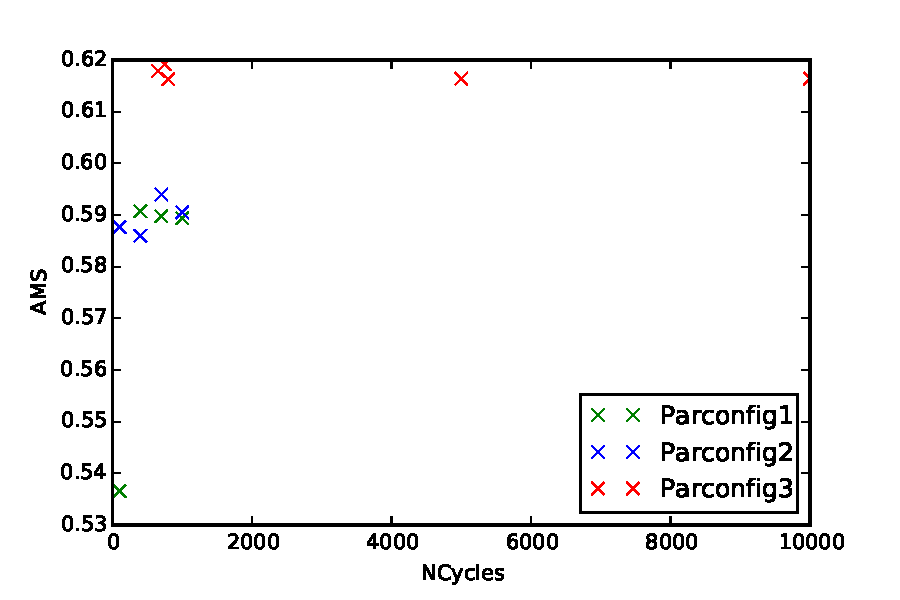
\includegraphics[width=\linewidth]{sections/parameter_optimization_ANN/plot5.pdf}
 		\caption[]{}
		\label{fig:NN_VariationofLayers}
  	  \end{subfigure} &
  	  \begin{subfigure}[b]{0.5\linewidth}
  	  	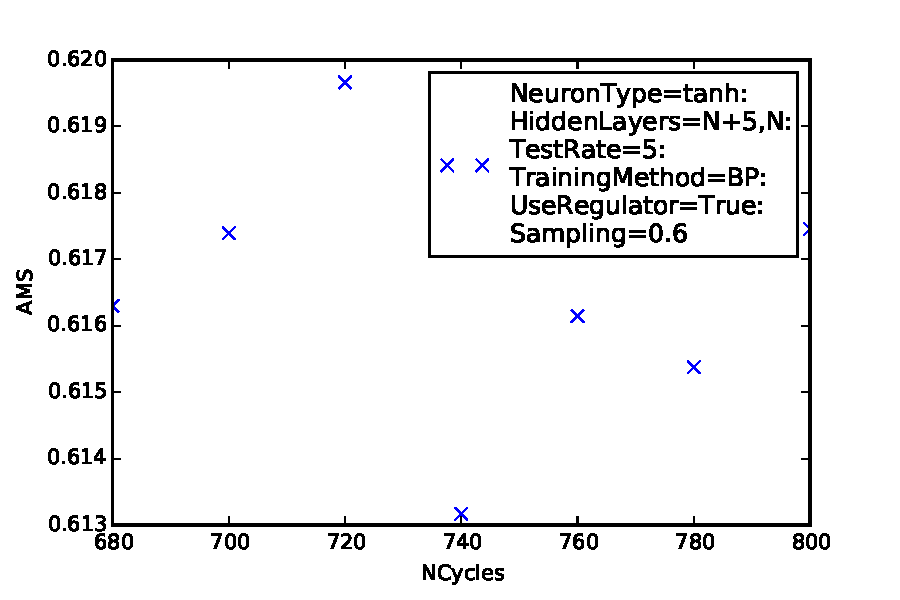
\includegraphics[width=\linewidth]{sections/parameter_optimization_ANN/plot4.pdf}
 		\caption[]{}
		\label{fig:NN_VariationofCycles}
  	  \end{subfigure}
  \end{tabular}
  \caption[]{AMS-Werte für die Parameter des Neuronalen Netzes. Jeder Punkt entspricht einem Training}
  \label{fig:AMS-distribution-plots}
\end{figure}



\noindent Es stellte sich heraus, dass die N+5,N layer Architektur minimal besser abschnitt und diese nun in den folgenden trainings verwendet wird. \\ \\
Um das Verhalten bei großen Anzahlen von Zyklendurchläufen zu untersuchen wurde zusätzlich bei einem Sampling=0.6 die Cycles=650,750,800,5000,10000 ausgewertet (siehe \ref{fig:NN_VariationofLayers}, rote Punkte). Eine signifikante Erhöhung der Cycle Anzahl hatte zwar eine rießige Laufzeitverlängerung zur Auswirkung, aber keine Verbesserung des AMS; im Gegenteil dieser hatte sich sogar minimal verschlechtert. \\ \\
Im Folgenden wurde der Bereich um NCycles = 700 näher untersucht, da vermutet wurde, dass dort der AMS am besten ist. Hierzu wurden die NCycles=800,780,760,740,720,700,680 mit einem Sampling=0.6 simuliert (siehe \ref{fig:NN_VariationofCycles}). Da diese Abbildung noch keinen Schlussfolgerungen zulässt wurde in dem darauffolgenden Schritt die Schrittgröße der NCycles verringert und erneut ausgewertet (dieses Mal unter Verwendung des vollen Trainings- und Testdatensatzes, Sampling=1) (siehe \ref{fig:NN_Variationlowstep}). 
\begin{figure}[tb]
\centering
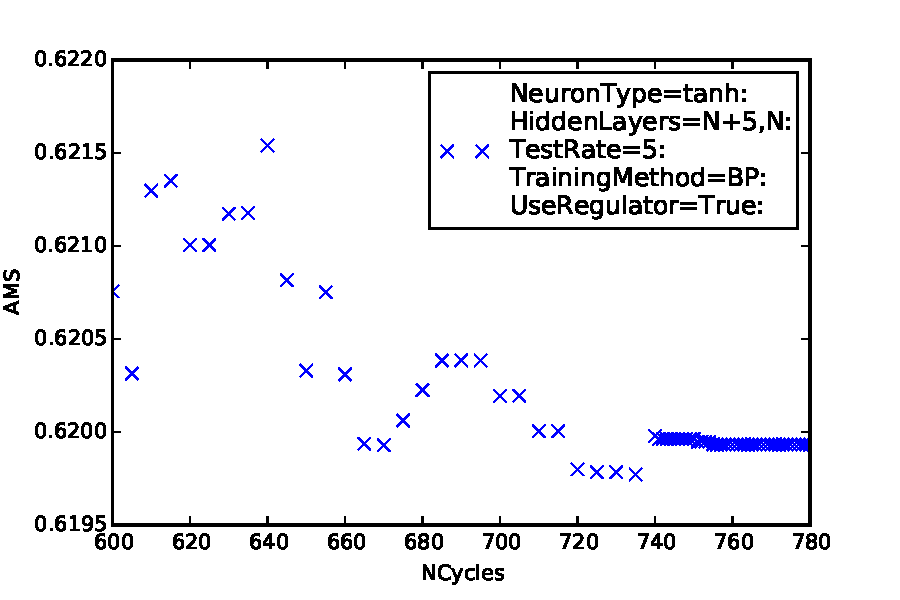
\includegraphics[scale=1]{sections/parameter_optimization_ANN/plot6.pdf}
\caption{AMS-Werte über NCycles}
\label{fig:NN_Variationlowstep} 
\end{figure}
Es stellte sich heraus, dass der AMS bei NCycles$\approx$640 den größten Wert von 0.6215 annimmt. Da dieser Wert jedoch bei Weitem nicht mit dem des BDT mithalten kann, wurde das NN als Methode verworfen. \\ \\